19. $y=\cfrac{x^2+7x+6}{x+|x+2|}=\begin{cases}\cfrac{(x+6)(x+1)}{2x+2},\ x\geqslant-2,\\ \cfrac{(x+6)(x+1)}{-2},\ x<-2.\end{cases}=
\begin{cases}\cfrac{x+6}{2},\ x\geqslant-2,\ x
eq-1,\\ -\cfrac{1}{2}x^2-\cfrac{7}{2}x-3,\ x<-2.\end{cases}$
$$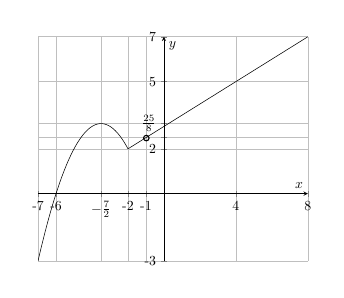
\begin{tikzpicture}[scale=0.5]
\begin{axis}[
    axis lines = middle,
    grid=major,
    legend pos={south west},
    xlabel = {$x$},
    %xlabel style={below right},
    ylabel = {$y$},
    xtick={-7, -6, -3.5,-2,-1, 4,8},
    xticklabels={-7, -6, $-\frac{7}{2}$,-2,-1, 4,8},
    ytick={-3, 3.125,2,2.5, 5,7},
    yticklabels={-3,$\frac{25}{8}$,2,$ $,5,7},
                  ]
	\addplot[domain=-7:-2, samples=100, color=black] {(x*x+7*x+6)/(-2)};
    \addplot[domain=-2:8, samples=100, color=black] {(x+6)/2};
	%\addlegendentry{$\text{Рис. 1}$};
\end{axis}
\draw (2.75,3.12) circle (2pt);
%\draw (3.7,3.05) circle (2pt);
\end{tikzpicture}$$
